%用来打印中文
\documentclass[UTF8]{ctexart}
\RequirePackage{iftex}
\RequirePackage{fix-cm}
\RequirePackage{fixltx2e}
%页面设置
\RequirePackage{geometry}
\if@twoside
 \geometry{a4paper,
 bindingoffset = 2cm,
 inner = 0.5cm,
 outer = 2cm,
 top = 3cm,
 bottom = 2cm
 }
\else
 \geometry{a4paper,
 left = 2cm,
 right = 2cm,
 top = 2cm,
 bottom = 2cm
 }
%各种包
\usepackage{fancyhdr}
\usepackage{amssymb}
\RequirePackage{graphicx}
\RequirePackage{subfigure}
\RequirePackage{caption}
\RequirePackage{diagbox}
\RequirePackage{multirow}
\RequirePackage{makecell}
\RequirePackage{booktabs}
%\usepackage{lipsum}
\usepackage{mathtools}
\usepackage{listings}%代码
%矩阵
\usepackage{amsmath,xcolor}
\RequirePackage{longtable}
\RequirePackage{array}
%页眉
\RequirePackage{float}
\RequirePackage{flowchart}
\pagestyle{fancy}
\renewcommand{\headrulewidth}{0.5pt} 
\lhead{} \rhead{name\ number}%\thepage
% 顶格写\noindent
\begin{document}
%\pagenumbering{arabic}
\section*{Information Theory Homework-1}
%姓名(学号)第二章作业.pdf
\begin{center}
\today
\end{center}
\subsection*{Assignments}

2.2,\ 2.3,\ 2.4,\ 2.10,\ 2.12,\ 2.21,\ 2.27,\ 2.28,\ 2.29,\ 2.31,\ 2.33,\ 2.34,\ 2.35,\ 2.42,\ 2.45.
\subsection*{2.2•函数的熵}

(a)$Y=2^X$ \ 函数为单射函数,故对任意$x_i \in \chi $, 有$p(x_i)=p(y_i)$,则$H(X)=H(Y)$


(b)$Y=cosX$\ 有$y\in [-1, 1]$,由余弦函数性质得到,根据x取值范围,函数可能单射也可能非单射,故$H(X)\geqslant H(Y)$, 当且仅当在X定义域内该函数满足单射时等号成立。


\subsection*{2.3•最小熵}

$H(\textbf{p})=-\sum p_ilogp_i$,由$H(X)\geqslant 0$知$H(\textbf{p})$最小值为0;

由$0\leqslant p_i \leqslant 1$,$0log0 = 0, 1log1=0, -p_ilogp_i > 0 (p_i \neq 0,1)$得使H(\textbf{p})取0的\textbf{p}有n个,且$\textbf{p}=(p_1, p_2, p_3, \dots ,p_n)$(其中有唯一$p_i=1(1\leqslant i \leqslant n)$,其他均为0)

\subsection*{2.4•随机变量的函数的熵}
由链式法则知(a),(c)成立;由g(X)为X函数知每个x均存在对应的g(x),即H(g(X)|X)=0,则(b)成立;同理,由函数定义知,每个g(x)存在至少一个对应的x,故H(X|g(X))$\geqslant$0,则(d)成立,得证H(g(X))$\leqslant$H(X).

\subsection*{2.10•不相交组合的熵}

(a)
\begin{equation*}
\label{eq:5-5}
\begin{split}
H(X)&=-\sum_i \alpha p_{1}(x_{1i})log\alpha p_{1}(x_{1i})-\sum_j (1-\alpha) p_{2}(x_{2j})log(1-\alpha)p_{2}(x_{2j})\\
&=- \alpha\sum_i p_{1}(x_{1i})logp_{1}(x_{1i})-(1-\alpha)\sum_j p_{2}(x_{2j})logp_{2}(x_{2j})-\alpha\sum_i p_{1}(x_{1i})log\alpha-(1-\alpha)\sum_j p_{2}(x_{2j})log(1-\alpha)\\
&=- \alpha\sum_i p_{1}(x_{1i})logp_{1}(x_{1i})-(1-\alpha)\sum_j p_{2}(x_{2j})logp_{2}(x_{2j})-\alpha log\alpha-(1-\alpha)log(1-\alpha)\\
&=\alpha H(X_1)+(1-\alpha)H(X_2)-\alpha log\alpha-(1-\alpha)log(1-\alpha)
\end{split}
\end{equation*}
(b)当a=0时,$H(X)=H(X_2)$,由$H(X_1),H(X_2)\geqslant 0$得$2^{H(X)}\leqslant 2^{H(X_1)}+2^{H(X_2)}$显然成立;同理,当a=1时,$H(X)=H(X_1)$,$2^{H(X)}\leqslant 2^{H(X_1)}+2^{H(X_2)}$显然成立;当$a\in (0,1)$时,对(a)中得到的H(X)表达式关于$\alpha$求导数,得
\begin{equation*}
\begin{split}
H(X)\prime &=H(X_1)-H(X_2)-log\alpha +log(1-\alpha)\\
&= H(X_1)-H(X_2)-log\frac{1-\alpha}{\alpha}\\
&= H(X_1)-H(X_2)-log(\frac{1}{\alpha}-1)
\end{split}
\end{equation*}
显然,在$\alpha \in (0,1)$时H(X)一阶导数为单调递减函数,由$H(X)\prime|_{\alpha=0^+}=+\infty, H(X)\prime|_{\alpha=1^-}=- \infty$知一阶导数存在零点$\alpha _0$有
\begin{equation}
\label{eq:1}
log(1-\alpha_0)-log\alpha_0 = H(X_2)-H(X_1)
\end{equation}
且$\alpha _0$对应H(X)极大值$H(X)_{max}=H(X_2)-log(1-\alpha _0)$,则有$$2^{H(X)}_{max}=2^{H(X_2)-log(1-\alpha _0)}=\frac{2^{H(X_2)}}{1-\alpha _0}$$
将式\ref{eq:1}代入$2^{H(X_1)}+2^{H(X_2)}$得
\begin{equation*}
\label{eq:2}
\begin{split}
2^{H(X_1)}+2^{H(X_2)}&=2^{H(X_2)-log(1-\alpha_0)+log\alpha _0}+2^{H(X_2)}\\
&=2^{H(X_2)}\times (1+\frac{\alpha_0}{1-\alpha _0})\\
&=\frac{1}{1-\alpha _0}2^{H(X_2)}\\
&=2^{H(X)}_{max}
\end{split}
\end{equation*}
则有$2^{H(X)}\leqslant 2^{H(X_1)}+2^{H(X_2)}$,当且仅当$log(1-\alpha_0)-log\alpha_0 = H(X_2)-H(X_1)$时等号成立,得证。
\subsection*{2.12•联合熵的例子}

(a)

\begin{displaymath}
H(X)=\frac{2}{3}log\frac{3}{2}+\frac{1}{3}log3\approx 0.918bit
\end{displaymath}
\begin{displaymath}
H(Y)=\frac{1}{3}log3+\frac{2}{3}log\frac{3}{2}\approx 0.918bit
\end{displaymath}

(b)
\begin{displaymath}
H(X|Y)=\frac{1}{3}\times 0 + \frac{2}{3}\times (\frac{1}{2}log2+\frac{1}{2}log2)=\frac{2}{3}bit
\end{displaymath}
\begin{displaymath}
H(Y|X)=\frac{2}{3}\times(\frac{1}{2}log2 + \frac{1}{2}log2)+\frac{1}{3}\times 0 = \frac{2}{3}bit
\end{displaymath}

(c)
\begin{displaymath}
H(X,Y) = H(X)+H(Y|X)\approx 1.58bit
\end{displaymath}

(d)

\begin{displaymath}
H(Y)-H(Y|X)\approx 0.25bit
\end{displaymath}

(e)

\begin{displaymath}
I(X;Y)=H(Y)-H(Y|X)\approx 0.25bit
\end{displaymath}

(f)如图1所示。
\begin{figure}[h]
    \centering
    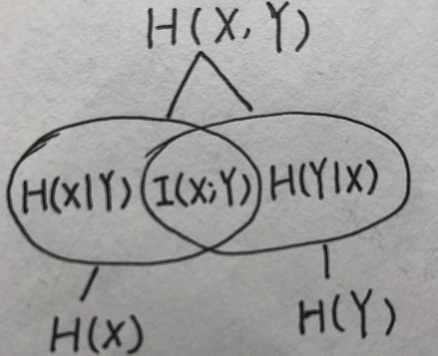
\includegraphics[totalheight=1.8in]{hw1_1.png}
    \caption{2.12(f)}
    \label{fig:2-12-f}
\end{figure}
\subsection*{2.21•概率的马尔可夫不等式}
设p(x)为概率密度函数。证明对任意的$d\geqslant 0$有$Pr\{p(X)\leqslant d\}log\frac{1}{d}\leqslant H(X)$

证明:
\begin{displaymath}
Pr\{p(X)\leqslant d\} = \sum_{p(x_i)\leqslant d}p(x_i)
\end{displaymath}
\begin{displaymath}
H(X)= \sum_{p(x_i)\leqslant d}p(x_i)log\frac{1}{p(x_i)}+ \sum_{p(x_j)> d}p(x_j)log\frac{1}{p(x_j)}\geqslant \sum_{p(x_i)\leqslant d}p(x_i)log\frac{1}{p(x_i)}
\end{displaymath}
\begin{equation*}
\begin{split}
Pr\{p(X)\leqslant d\}log\frac{1}{d}&=\sum_{p(x_i)\leqslant d}p(x_i)log\frac{1}{d}\\
&\leqslant\sum_{p(x_i)\leqslant d}p(x_i)log\frac{1}{p(x_i)}
\end{split}
\end{equation*}
$\therefore Pr\{p(X)\leqslant d\}log\frac{1}{d}\leqslant H(X)$
\subsection*{2.27•熵的组合法则}
证明:
\begin{equation*}
\begin{split}
H(\textbf{p})&=\sum _{i=1}^{m}p_ilog\frac{1}{p_i}\\
&=H(\textbf{q})-(p_{m-1}+p_m)log\frac{1}{p_{m-1}+p_m}+p_{m-1}log\frac{1}{p_{m-1}}+p_mlog\frac{1}{p_m}\\
&=H(\textbf{q})-p_{m-1}log\frac{p_{m-1}}{p_{m-1}+p_m}-p_mlog\frac{p_m}{p_{m-1}+p_m}\\
&=H(\textbf{q})+(p_{m-1}+p_m)[-\frac{p_{m-1}}{p_{m-1}+p_m}log\frac{p_{m-1}}{p_{m-1}+p_m}-\frac{p_{m}}{p_{m-1}+p_m}log\frac{p_m}{p_{m-1}+p_m}]\\
&=H(\textbf{q})+(p_{m-1}+p_m)H(\frac{p_{m-1}}{p_{m-1}+p_m},\frac{p_m}{p_{m-1}+p_m})
\end{split}
\end{equation*}

\subsection*{2.28•混合使熵增加}

设原概率分布为\textbf{$p_1$},调整后为\textbf{$p_2$},则有
\begin{equation*}
\begin{split}
H(P_1)-H(P_2)&=-p_ilogp_i-p_jlogp_j+2\times \frac{p_i+p_j}{2}log\frac{p_i+p_j}{2}\\
&=-p_ilogp_i-p_jlogp_j+(p_i+p_j)log\frac{p_i+p_j}{2}\\
\end{split}
\end{equation*}
由对数和不等式得$H(P_1)-H(P_2)\leqslant 0$即$H(P_1)\leqslant H(P_2)$,变换后熵增加。

更加一般的证明:

假设原分布为\textbf{$p_1$},其中两概率值为$p_i,p_j$,设$p_i\geqslant p_j,p_i+p_j=a$,作调整使$$p_i\prime = p_i-\delta, p_j\prime = p_j+\delta(0\leqslant\delta\leqslant \frac{p_i-p_j}{2} )$$
记调整后为\textbf{$p_3$}
\begin{equation*}
\begin{split}
H(P_1)-H(P_3)&=-p_ilogp_i-p_jlogp_j + (p_i-\delta)log(p_i-\delta) + (p_j+\delta)log(p_j+\delta)\\
&=  -p_ilogp_i-(a-p_i)log(a-p_i) + (p_i-\delta)log(p_i-\delta) + (a-p_i+\delta)log(a-p_i+\delta)\\
\end{split}
\end{equation*}
记$f(p)=-plogp-(a-p)log(a-p)$,则有
\begin{equation*}
\begin{split}
f^\prime (p)&=-logp -1 + log(a-p) + 1\\
&= -logp + log(a-p)\\
&= log(\frac{a}{p}-1)\\
\end{split}
\end{equation*}

显然,$f^\prime (p)$为单调递减函数,且$\lim_{p \to 0}f^\prime (p)=+\infty,\  \lim_{p \to a}f^\prime (p) = -\infty, \ f^\prime (\frac{a}{2})=0,$则f(p)在(0,a)上先单调增后单调减且在$p=\frac{a}{2}$时取得极大值,即$p_i$越靠近$\frac{a}{2}$该函数值越大,则$H(P_1)-H(P_3)\leqslant 0$,即调整后熵增大,若有多个概率改变,可分为多次两两一组的概率改变,得证。
\subsection*{2.29•不等式}

(a)
\begin{equation*}
\begin{split}
H(X,Y|Z)&=H(X|Z)+H(Y|X,Z)\\
H(Y|X,Z)& \geqslant 0\\
\therefore H(X,Y|Z)&\geqslant H(X|Z)
\end{split}
\end{equation*}

当且仅当H(Y|X,Z)=0时等号成立。

(b)
\begin{equation*}
\begin{split}
I(X,Y;Z)&=I(X;Z)+I(Y;Z|X)\\
I(Y;Z|X)& \geqslant 0\\
\therefore I(X,Y;Z)&\geqslant I(X;Z)
\end{split}
\end{equation*}

当且仅当I(Y;Z|X)=0时等号成立。


(c)
\begin{equation*}
\begin{split}
H(X,Y,Z)-H(X,Y)&=H(X)+H(Y|X)+H(Z|X,Y)-H(X)-H(Y|X)\\
&=H(Z|X,Y)\\
&=H(Z|X)-I(Y|X;Z)\\
H(X,Z)-H(X)&=H(X)+H(Z|X)-H(X)\\
&=H(Z|X)\\
\end{split}
\end{equation*}

$$I(Y|X;Z) \geqslant 0$$

$$\therefore H(X,Y,Z)-H(X,Y)\leqslant H(X,Z)-H(X)$$

当且仅当$I(Y|X;Z)=0$时等号成立。

(d)

$$I(X;Z|Y)+I(Y;Z)=I(Y;Z|X)+I(X;Z)$$

$$\therefore I(X;Z|Y)=I(Y;Z|X)+I(X;Z)-I(Y;Z)$$

等号恒成立。


\subsection*{2.31•条件熵}

由题意,X,Y,g(Y)构成马尔可夫链$X\rightarrow Y\rightarrow g(Y)$,则有
\begin{equation}
I(X;Y)\geqslant I(X;g(Y))
\end{equation}
当且仅当X,g(Y),Y构成马尔可夫链$X\rightarrow g(Y)\rightarrow Y$时等号成立;

由$I(X;Y)=H(X)-H(X|Y), I(X;g(Y))= H(X)-H(X|g(Y))$得当且仅当式2等号成立$X\rightarrow g(Y)\rightarrow Y$,即X,Y线性无关、g(Y)为单射函数时有H(X|Y)=H(X|g(Y))。

\subsection*{2.33•费诺不等式}

由题意有$\sum_{i=2}^m p_i=P_e, 1+P_e=1$,则
\begin{equation*}
\begin{split}
H(p)&= \sum _{i=1}^m p_ilog\frac{1}{p_i}\\
&=p_1log\frac{1}{p_1}+\sum_{i=2}^m p_ilog\frac{1}{p_i}\\
&=p_1log\frac{1}{p_1}+\sum_{i=2}^m P_e\frac{p_i}{P_e} (log\frac{P_e}{p_i}-logP_e)\\
&=p_1log\frac{1}{p_1} + P_eH(\frac{p_2}{P_e},\dots ,\frac{p_m}{P_e})-P_elogP_e\\
&=H(P_e)+ P_eH(\frac{p_2}{P_e},\dots ,\frac{p_m}{P_e})\\
&\leqslant H(P_e)+ P_elog(m-1)\\
\end{split}
\end{equation*}

$\therefore H(p)_{max}=H(P_e)+ P_elog(m-1)$,在$p_2=p_3=\dots=p_m=\frac{P_e}{m-1}$时取等号。

由$H(P_e)= p_1log\frac{1}{p_1}+p_elog\frac{1}{p_e}\leqslant 1$,得$$P_e\geqslant \dfrac{H(p)-1}{log(m-1)}$$


\subsection*{2.34•初始条件熵}

由数据处理不等式$I(X_0;X_n)\geqslant I(X_0;X_{n+1})$,则$$H(X_0)-H(X_0|X_n)\geqslant H(X_0)-H(X_0|X_{n+1})$$即$$H(X_0|X_n)\leqslant H(X_0|X_{n+1}) $$

$\therefore H(X_0|X_n)$随n非减。


\subsection*{2.35•相对熵是不对称的}

$H(p)=\frac{1}{2}log2+\frac{1}{4}log4+\frac{1}{4}log4=\frac{3}{2}$

$H(q)=3\times\frac{1}{3}log3=log3$

$$D(p||q)=\sum _{x\in\chi}p(x)log\dfrac{p(x)}{q(x)}\approx 0.085$$

$$D(q||p)=\sum _{x\in\chi}q(x)log\dfrac{q(x)}{p(x)}\approx 0.082$$

$$\therefore D(p||q)\neq D(q||p) $$

\subsection*{2.42•不等式}

(a)$H(5X)=H(X)$

(b)$I(g(X);Y)\leqslant I(X;Y) $

(c)$H(X_0|X_{-1})\geqslant H(X_0|X_{-1},X_1) $

(d)$\dfrac{H(X,Y)}{H(X)+H(Y)} \leqslant 1$

\subsection*{2.45•有限熵}

证明:对于离散随机变量$X=\{1,2,\cdots\}$,如果$ElogX<\infty$,则$H(X)<\infty$。

证:不妨设X中共有m个元素,
\begin{equation*}
\begin{split}
H(X)&=\sum_{n=1}^m p_nlog\frac{1}{p_n}\\
&\leqslant m\frac{1}{m}logm\\
&=logm\\
ElogX&\leqslant logEX\\
&=log\frac{m-1}{2}\leqslant \infty\\
\therefore logm&<\infty\\
\therefore H(X)&<\infty
\end{split}
\end{equation*}
\end{document}
